\documentclass[9pt]{beamer}

\usepackage[utf8x]{inputenc}

\usetheme{Ampang}
\usecolortheme{ampangcolor}
%\usecolortheme{warna}

%%% XeLaTeX engine for Ubuntu Font support
\usepackage{xltxtra}
\setsansfont[
BoldFont=Ubuntu-Bold.ttf,
ItalicFont=Ubuntu-Italic.ttf,
BoldItalicFont=Ubuntu-BoldItalic.ttf
]
{Ubuntu-Regular.ttf}
\setmonofont{UbuntuMono-Regular.ttf}

\usepackage{listings}

\lstset{basicstyle=\ttfamily\footnotesize}
\makeatletter
\def\verbatim@font{\footnotesize\ttfamily}
\makeatother

\title{Time delay estimation\\{\normalsize (case of gravitationally-lensed quasars)}}
\author{Saghar Asadi\\ Egil Moeller}
\date{\today}
%\institute{Share\LaTeX}

\begin{document}

\maketitle

\section{Outline}

\begin{frame}{Outline}
\begin{itemize}
  \item Question
  \item Dataset
  \item Main idea
  \item What we tried
  \begin{itemize}
    \item Unsuitable methods
    \item (probably) Suitable methods
  \end{itemize}
%  \item Metrics of success
  \item Current state
  \item Way to improvement
\end{itemize}
\end{frame}

\section{Question}

\begin{frame}{Question - Original}
  \begin{figure}
    \includegraphics[width=0.9\textwidth]{question-original.png}
  \end{figure}
  \hspace{0.33\textwidth}TimeDelayChallenge.org
\end{frame}

\begin{frame}{Question - Machine learning approach}
  \textbf{How much do the ground truth information mean in terms of accuracy?}\\
  \vspace{10mm}
  \textbf{OR:}\\
  %\vspace{10mm}
  \normalsize{How limiting are the intrinsic uncertainties?}\\
  \vspace{10mm}
  \textbf{Meta question:}\\
  %\vspace{10mm}
  \normalsize{What does this mean in terms of the Hubble constant?}
\end{frame}

\section{Dataset}

\begin{frame}{Dataset - Inroduction}
  Realistic mock observed lensed quasar light curves
\end{frame}

\begin{frame}{Dataset - AGN variability}
  \hspace{0.8\textwidth}\small{Dobler+2015}
  \begin{figure}
    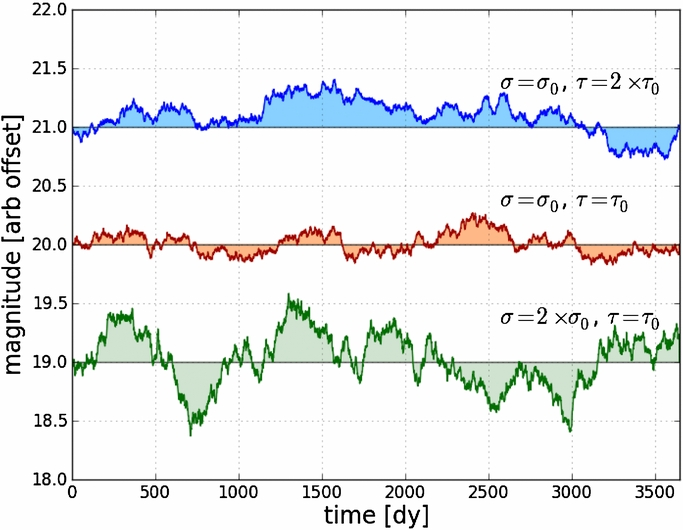
\includegraphics[width=0.9\textwidth]{dataset-original.jpg}
  \end{figure}
\end{frame}

\begin{frame}{Dataset - Microlensing effects}
  \hspace{0.57\textwidth}\small{Dobler+2015}
  \begin{figure}
    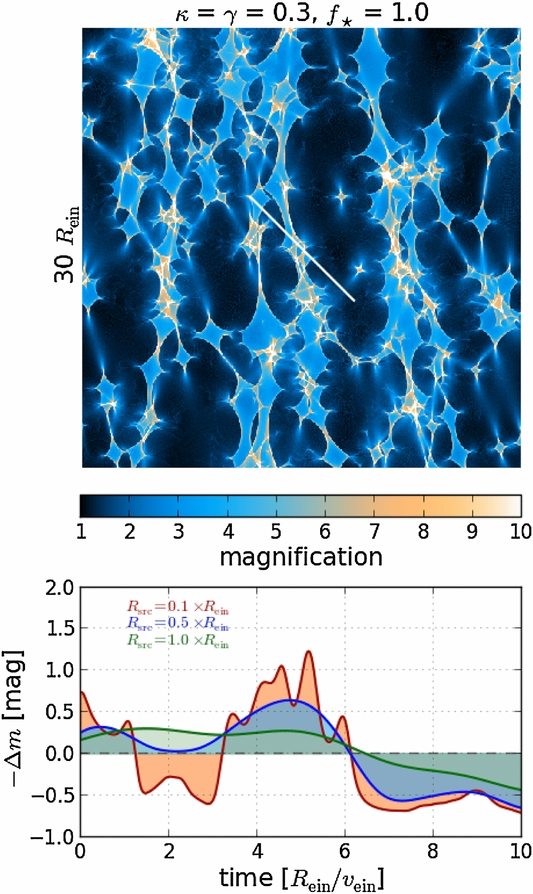
\includegraphics[width=0.45\textwidth]{dataset-microlensing.jpg}
  \end{figure}
\end{frame}

\begin{frame}{Dataset - Observational effects}
\hspace{0.82\textwidth}\small{Dobler+2015}
\begin{figure}
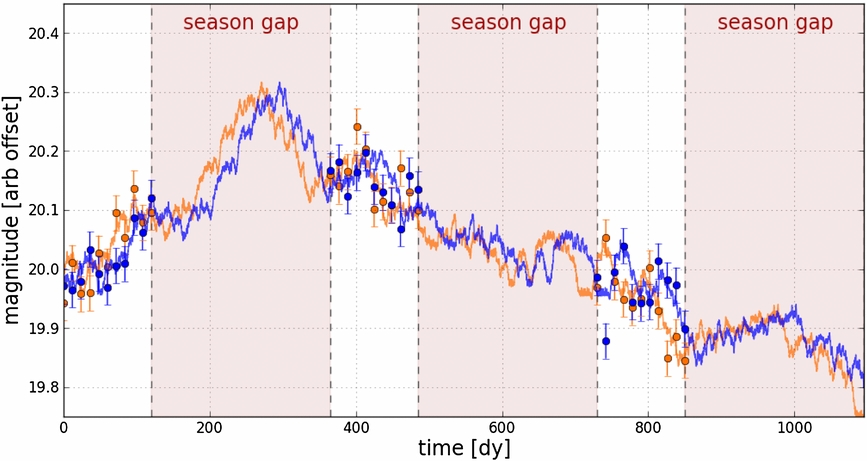
\includegraphics[width=0.95\textwidth]{dataset-season-gap.jpg}
\end{figure}
\end{frame}

\begin{frame}{Dataset}
  \hspace{0.85\textwidth}\small{Liao+2015}
  \begin{figure}
    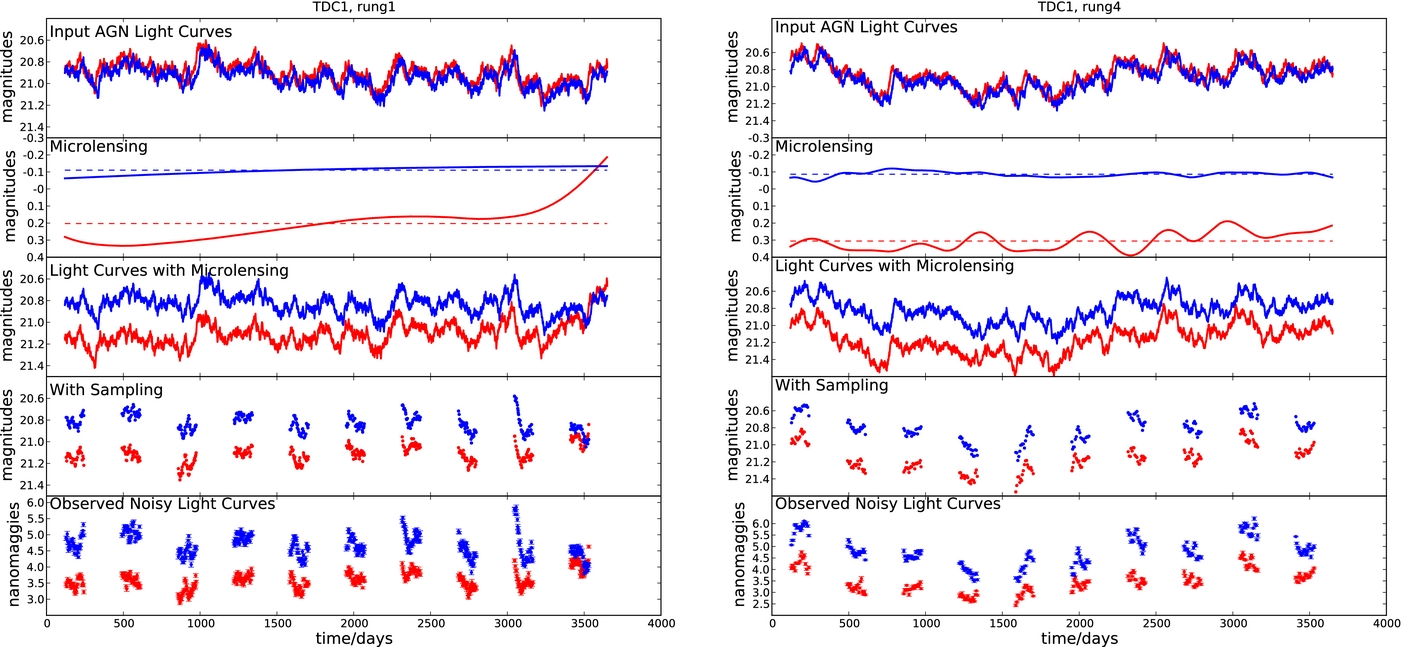
\includegraphics[width=0.95\textwidth]{dataset-total.jpg}
  \end{figure}
\end{frame}

\section{Main idea}
\begin{frame}[fragile]{Main idea}
\begin{itemize}
  \item {\bf Smooth} and {\bf interpolate} evenly sampled data
  \item {\bf Compare} two light curves of each window for dt between 0 and window length
  \begin{itemize}
    \item \lstinline{scipy.signal.correlate}
    \item MSE
  \end{itemize}
  \item Find the {\bf best timeshift} for each window
  \begin{itemize}
    \item \lstinline{max(correlate)}
    \item \lstinline{min(MSE)}
  \end{itemize}
  \item {\bf Compare} estimated best dt of different windows of the same pair
  \begin{itemize}
    \item \lstinline{np.median(dt[window])}
    \item \lstinline{np.mean(dt[window])}
    \item \lstinline{np.std(dt[window])}
    \item weighted mean (based on absolute correlate value)
  \end{itemize}
  \item Use a {\bf clustering} algorithm to reduce the noise
  \item Apply a {\bf regression} method to the clustered values
\end{itemize}
\end{frame}

\begin{frame}{Dataset - smooth (Gaussian processes)}
  \begin{figure}
    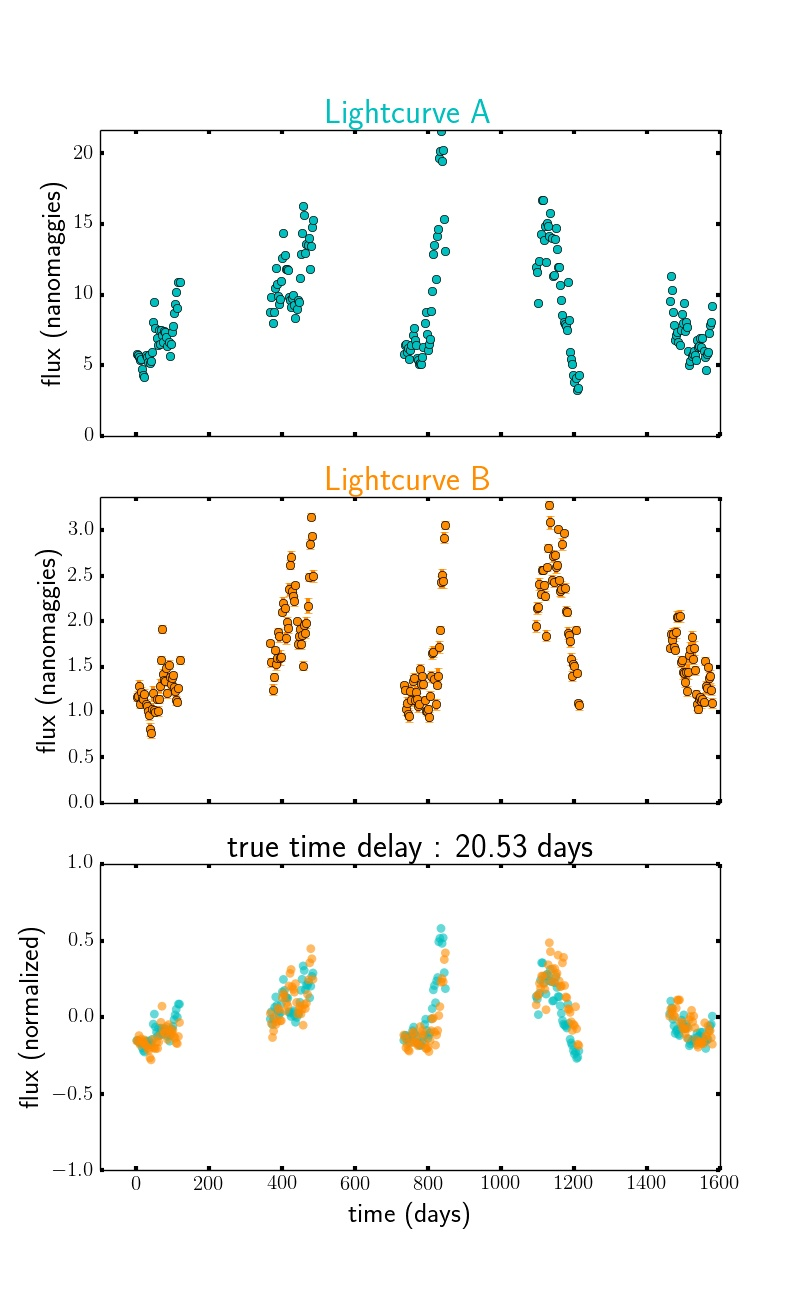
\includegraphics[width=0.45\textwidth]{Fig1.jpg}
    \hspace{0.05\textwidth}
    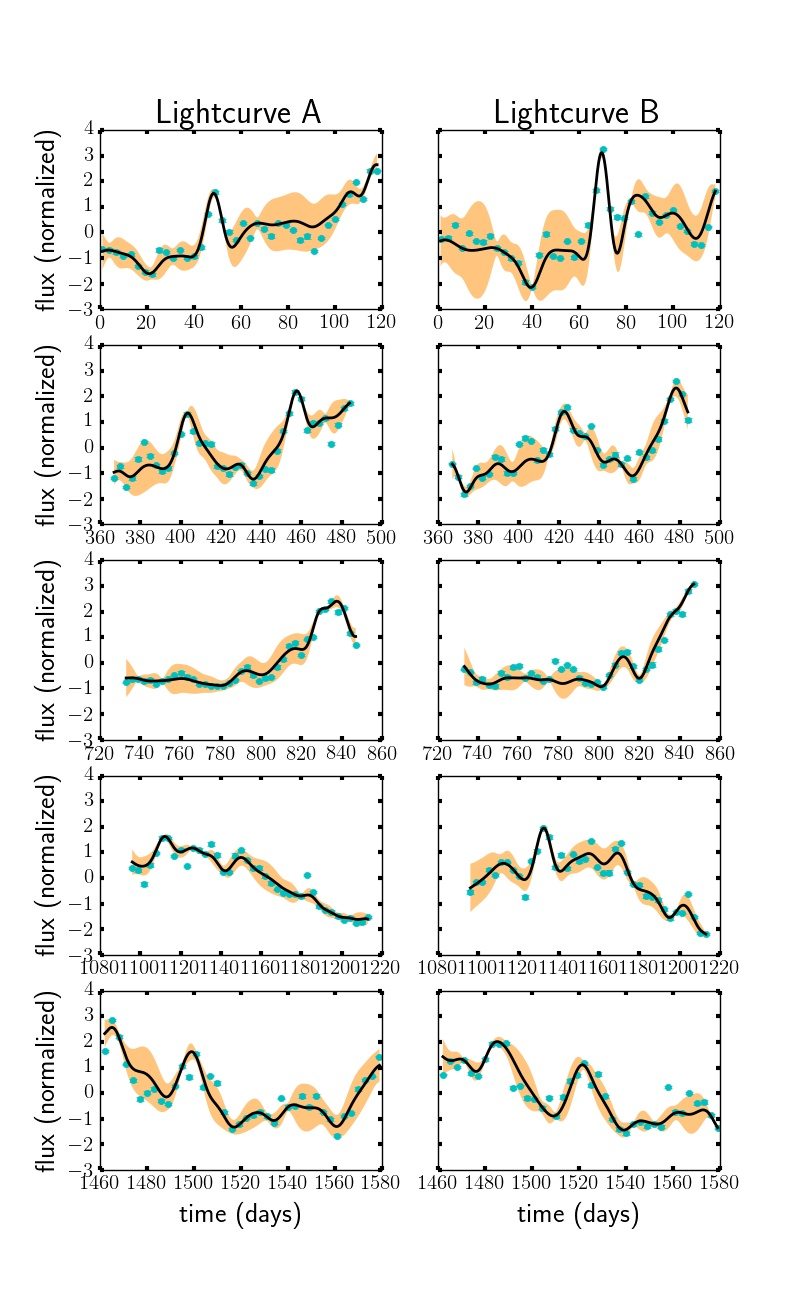
\includegraphics[width=0.45\textwidth]{Fig2.jpg}
  \end{figure}
\end{frame}

\begin{frame}[fragile]{Dataset - smooth (Gaussian processes)}
  \begin{verbatim}

    gp = GaussianProcess(corr = "squared_exponential",
                         regr = "quadratic",
                         theta0 = sigma,
                         thetaL = tau,
                         thetaU = tau,
                         nugget = (dy / y) ** 2,
                         random_start=500)


    gp.fit(X, y)

    y_pred, MSE = gp.predict(x, eval_MSE=True)

  \end{verbatim}
\end{frame}

\begin{frame}{Comparison - What we tried ... and failed}
  \begin{itemize}
    \item Lomb-Scargle periodogram on raw, unevenly-sampled data
    \item FFT on even resampling of the smooth models
  \end{itemize}
  {\bf Idea}: phase (angle of the complex FFT value) of the highest-amplitude frequency would correlate with the real dt.\\
  {\bf Problem}: Inside each window, the signal is highly a-periodic, which probably introduces a lot of noise.
\end{frame}

\begin{frame}{Comparison - What we tried ... and succeeded}
  \begin{figure}
    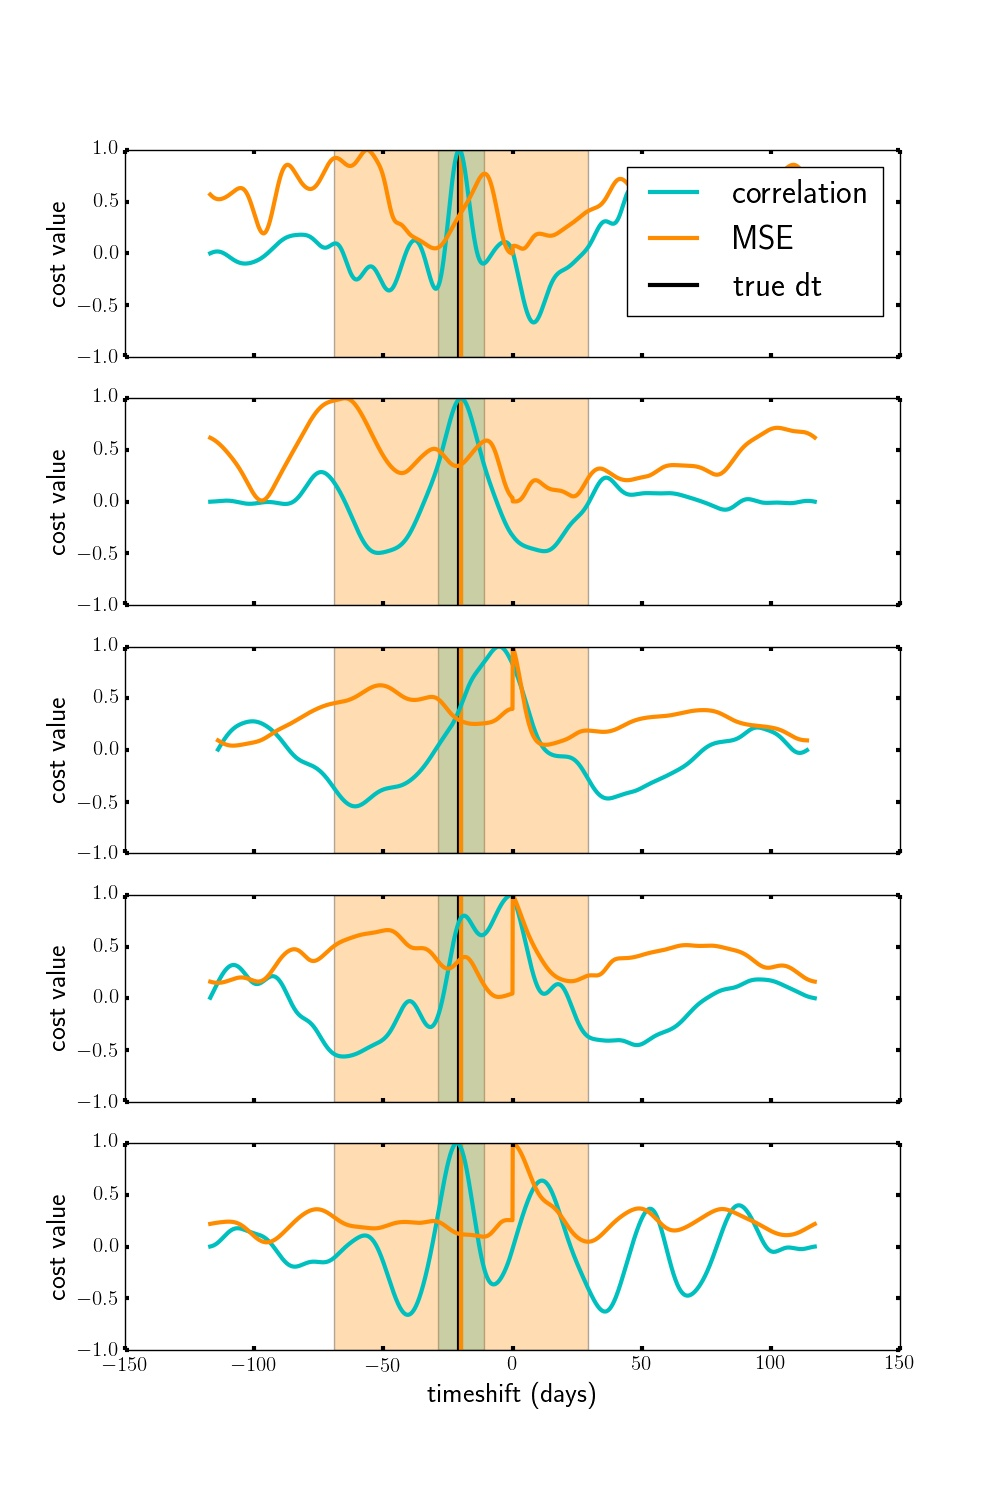
\includegraphics[width=0.45\textwidth]{Fig31.jpg}
    \hspace{0.05\textwidth}
    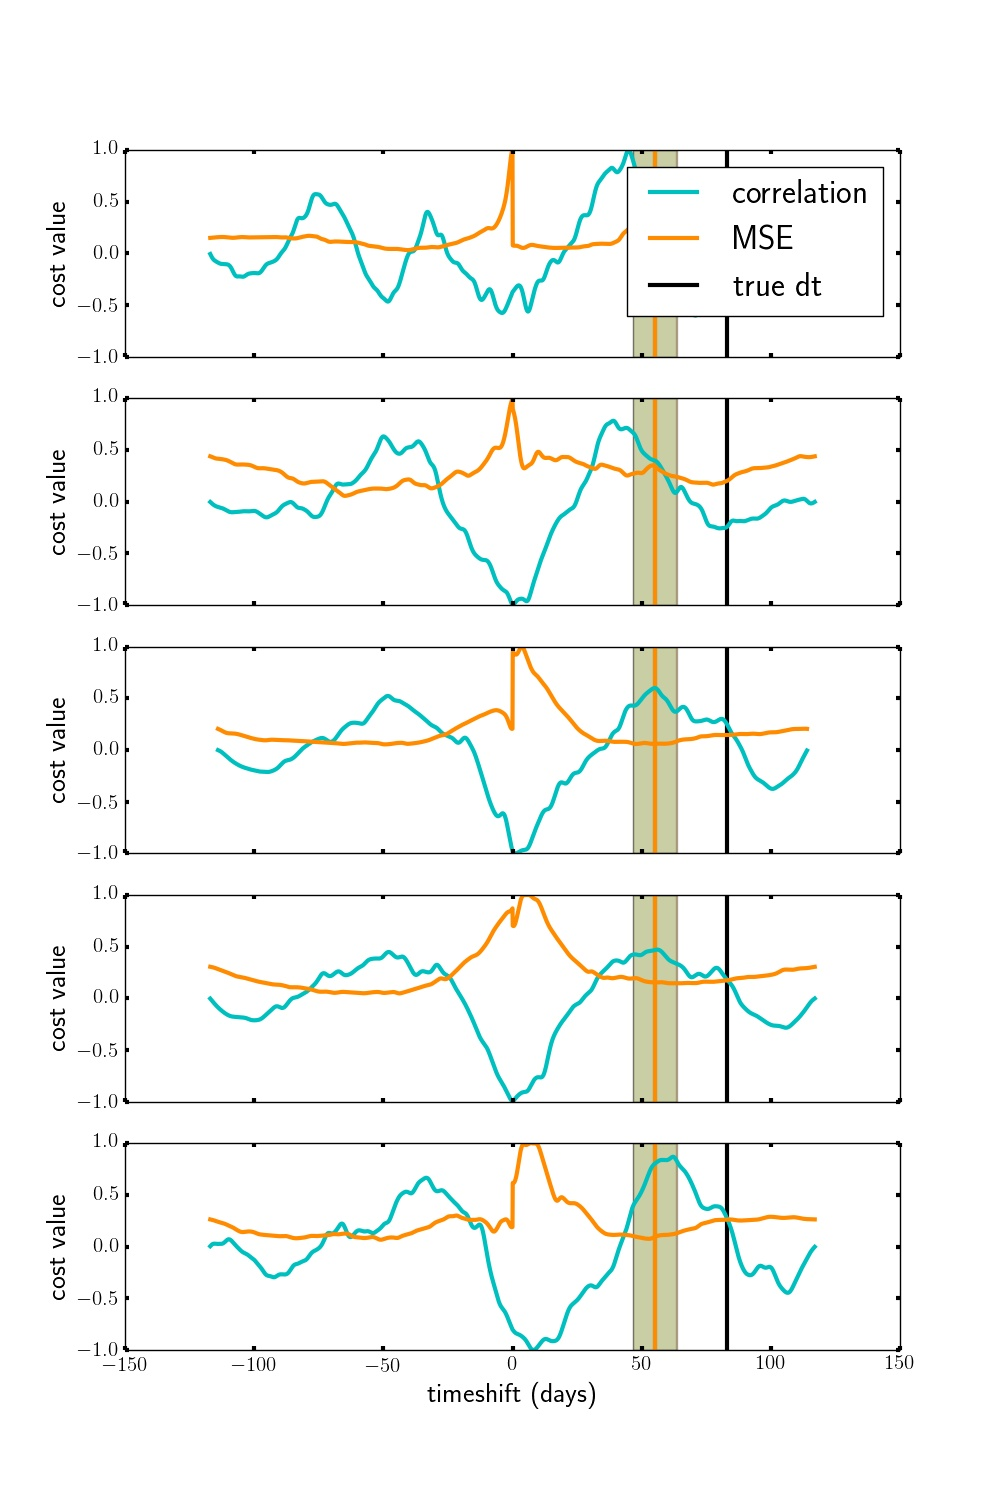
\includegraphics[width=0.45\textwidth]{Fig32.jpg}
  \end{figure}
\end{frame}

%% \section{Metrics of success}
%% \begin{frame}{Metrics of success}
%% \begin{columns}
%% \begin{column}{0.5\textwidth}  %%<--- here
%%     \begin{center}
%%       \begin{itemize}
%%         \item goodness-of-fit
%%         \item efficiency
%%         \item precision
%%         \item accuracy or bias
%%       \end{itemize}
%%      \end{center}
%% \end{column}
%% \begin{column}{0.5\textwidth}  %%<--- here
%%     \begin{center}
%%       \begin{itemize}
%%         \item $\chi^2$ < 1.5
%%         \item f > 0.5
%%         \item P < 0.03
%%         \item |A| < 0.03
%%       \end{itemize}
%%      \end{center}
%% \end{column}
%% \end{columns}
%% \end{frame}

\begin{frame}{Reduce noise - clustering}
  \begin{figure}
    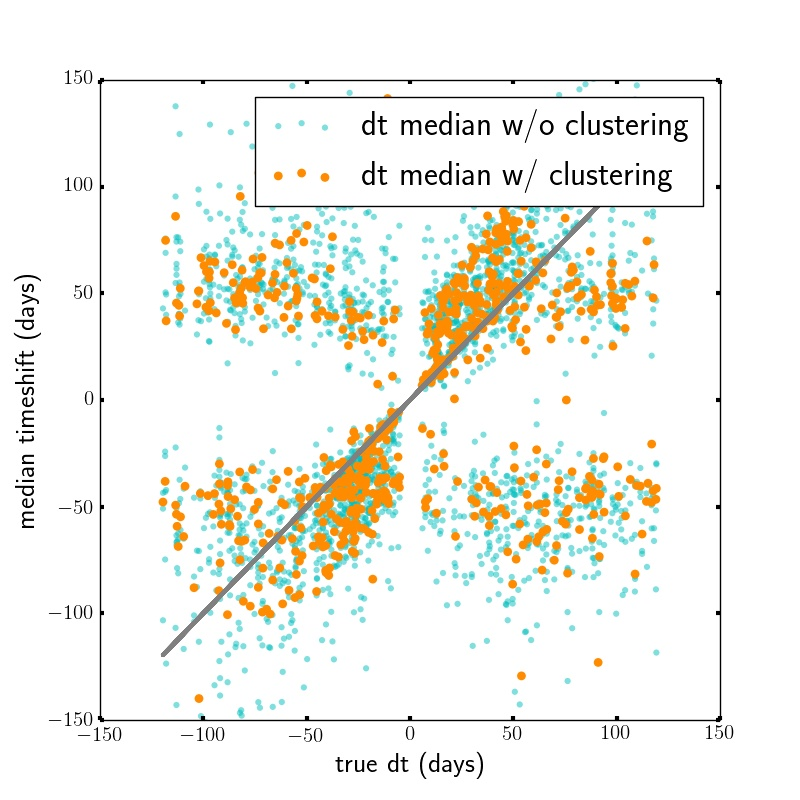
\includegraphics[width=0.65\textwidth]{Fig4.jpg}
  \end{figure}
\end{frame}

\section{Way to improvement}
  \begin{frame}{Way to improvement}
    \begin{itemize}
      \item Error analysis
      \item Regularized linear regression on correlation arrays
      \item Unsupervised learning
      \item Neural network
    \end{itemize}
\end{frame}

\section{Future progress}
\begin{frame}{Future progress}
  \hspace{0.33\textwidth}Follow the project on GitHub: \\
  \hspace{0.24\textwidth}https://github.com/asadisaghar/TimeDelay
\end{frame}

\end{document}
